\section{rSLA DSL}
\label{sec:dsl}
alphabet, vocabulary, language structure

production rules

\subsection{rSLA language structure, alphabet}

The rSLA language follows the semantic decomposition of the WSLA specification \cite{wsla}, where an SLA takes the form of a hierarchical tree with a single root node and numerous uni-directional edges. In an rSLA tree, the root node represents an SLA object. Figure \ref{rSLA_diag} illustrates diagrammatically the rSLA vocabulary as a tree of objects that the DSL implements. Listing \ref{lst} explains the rSLA tree using set notation to highlight the nesting that is inherited from the WSLA specification \cite{wsla}, between language objects:

\begin{minipage}{0.5\textwidth}
\begin{figure}[H]
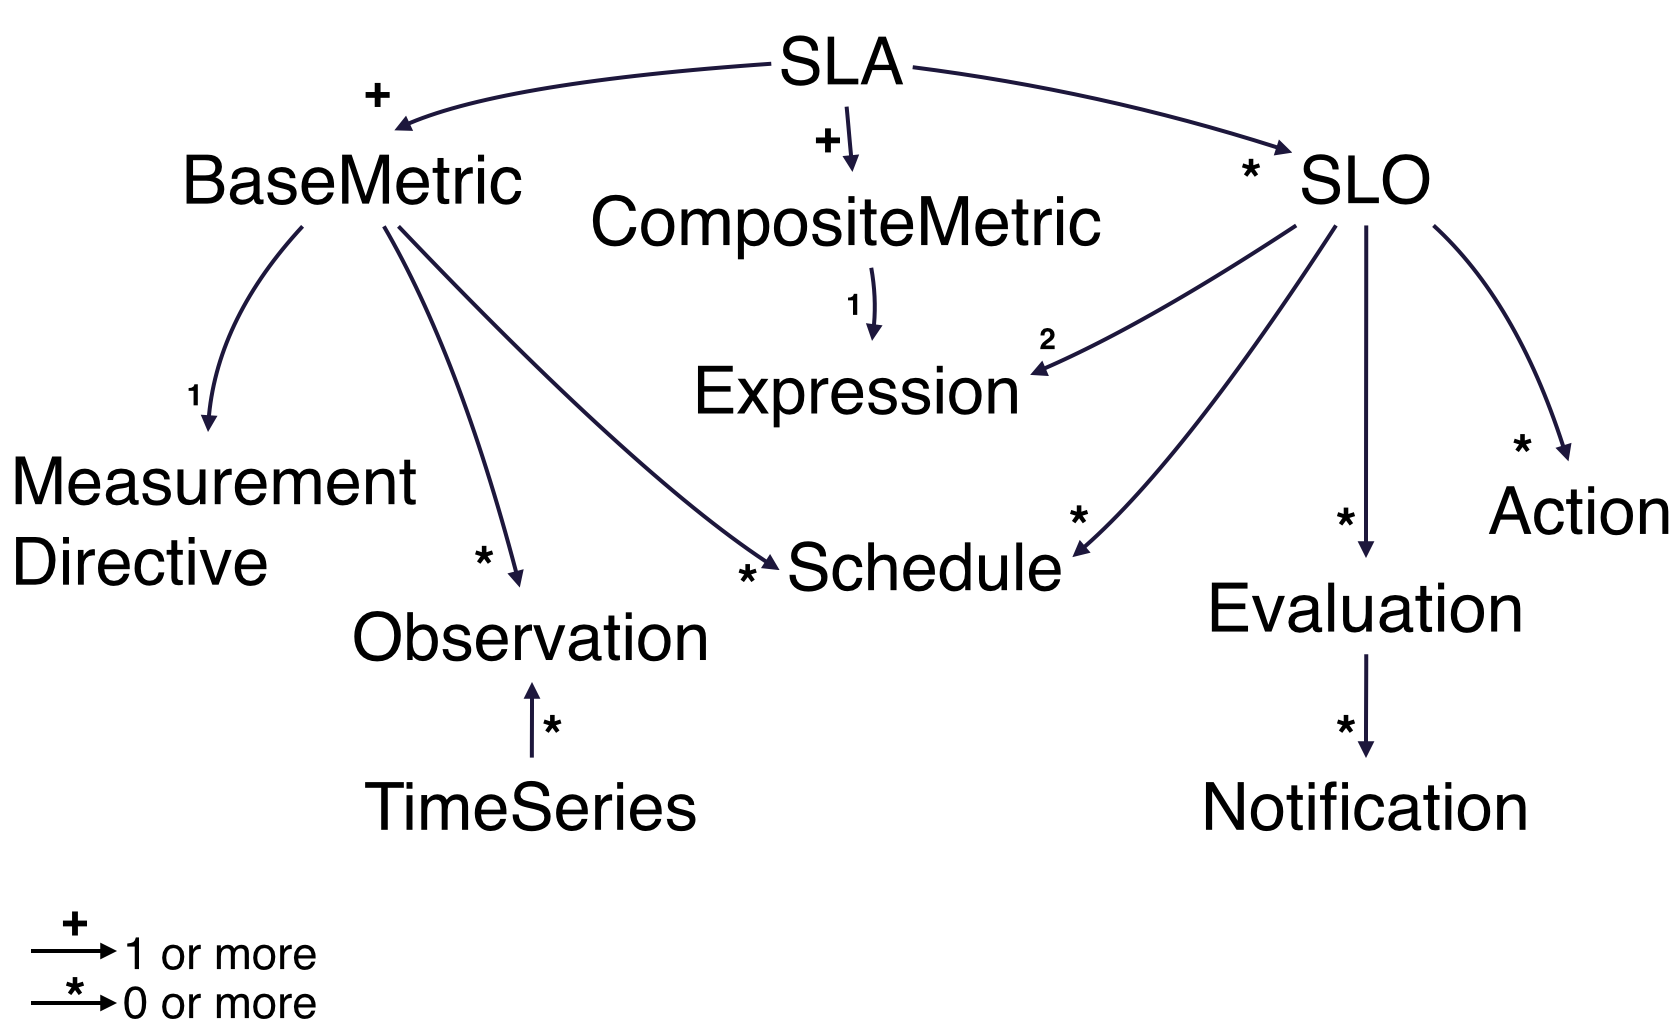
\includegraphics[width=1.0\textwidth]{pics/rslaobject}
\caption{\label{rSLA_diag} rSLA DSL object diagram}
\end{figure}
\end{minipage} \hfill
\begin{minipage}{0.5\textwidth}
\begin{lstlisting}[breaklines, mathescape, firstnumber=auto, caption=rSLA vocabulary, label=lst]
SLA $\supset$ { BaseMetric+, CompositeMetric*, SLO+ }
BaseMetric $\supset$ { MeasurementDirective, Observation*, Schedule* }
CompositeMetric $\supset$ { Expression* }
SLO $\supset$ { Expression*, Action*, Evaluation*, Schedule* }
\end{lstlisting}
\end{minipage}

Connections between nodes in the rSLA tree highlight nesting of SLA context. In Figure \ref{rSLA_diag} nodes that are close to the root, designate SLA branches like base, composite metrics and service level objectives. Edges between nodes are uni-directed to illustrate the rSLA tree hierarchy. The edge direction points to the nested element in the hierarchical relationship. $+$ symbols on edges indicate that the parent node may include multiple nested objects. Hence, an SLA may consist of multiple base, composite metrics as well as SLOs.



rSLA supports the creation of programming blocks that express SLA context and that are necessary to run and manage rSLAs in a cloud environment. 
In the rSLA language nested relationships denote inclusive associations between objects. For example, an SLA includes base and composite metrics as 
well as SLOs. Inclusive relationships of rSLA objects do not share same multiplicity rules (listing \ref{lst}). The rSLA DSL follows the WSLA 
specification \cite{wsla} with respect to the definition of rSLA objects and of their basic attributes.

In Figure \ref{rSLA_diag} the $Notification$ and $TimeSeries$ classes do not appear in the rSLA set representation. These two classes produce objects 
that help with service level management operations like the statistical analysis of data coming from monitoring or automated notification reports on 
scheduled events of service level evaluation. Such two classes are not initially required to build and run SLA instances in a cloud environment, but 
may be required while one or more SLA management tasks are processed.



conclude that
 
\subsection{rSLA language production rules}

rSLA language constructs: elements have relationships/dependencies, there is nesting and management dependencies

production rules